\usetikzlibrary{calc}

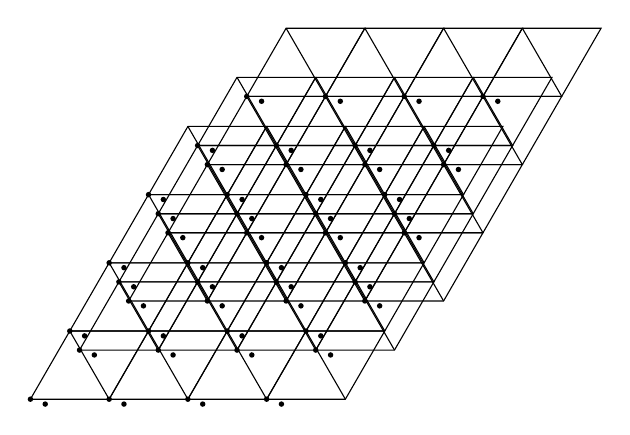
\begin{tikzpicture}[
        scale=1,
        every node/.style={fill, circle, inner sep=.7},
        %y={(-7mm, -7mm)},
        %x={(10mm, 0mm)},
        %z={(0mm, 10mm)},
    ]

    % Define Bravais lattice.
    \coordinate (a1) at (1, 0, 0);
    \coordinate (a2) at (.5, 0.866, 0);
    \coordinate (a3) at (0, 0, 1.62);

    % Define unit cell.
    \coordinate (u1) at (0, 0, 0);
    \coordinate (u2) at (.5, .25, .81);

    \foreach \a in {0,...,3}
    \foreach \b in {0,...,3}
    \foreach \c in {0,...,2}
    {
        \coordinate (x) at ($\a*(a1) + \b*(a2) + \c*(a3)$);

        \coordinate (xa1) at ($(x) + (a1)$);
        \coordinate (xa2) at ($(x) + (a2)$);
        \coordinate (xa3) at ($(x) + (a3)$);

        \coordinate (xa4) at ($(x) + (a1) + (a2)$);

        \coordinate (xu1) at ($(x) + (u1)$);
        \coordinate (xu2) at ($(x) + (u2)$);

        \draw (xu1) node {} ;
        \draw (xu2) node {};

        \draw (x) -- (xa1) -- (xa4) -- (xa2) -- (x);
        \draw (xa1) -- (xa2);
    }
\end{tikzpicture}
